\chapter{Diseño y Desarrollo del Prototipo}
\par 
El siguiente capítulo hablaremos de los pasos a seguir para la elaboración del prototipo de dispositivo de medición de temperatura. Elegiremos ciertos componentes mencionados en el marco teórico; ya que cumplen con ciertas características que necesitamos o simplemente porque presentan un mayor valor agregado al prototipo. El principal componente de nuestro prototipo es nuestra placa Arduino la cual brinda componentes adicionales al microcontrolador como un regulador de voltaje y un convertidor serial a USB, muy útil al momento de programar nuestro prototipo. Otras de las razones por la cual utilizamos Arduino son\cite{arduino-intro}:

\begin{itemize}
	\item Económico: 
	Las placas Arduino son relativamente económicas en comparación con otras plataformas de microcontroladores. La versión menos costosa del módulo Arduino se puede ensamblar a mano, e incluso los módulos Arduino premontados cuestan menos de \$50.
	
	\item Multiplataforma: El software Arduino (IDE) se ejecuta en sistemas operativos Windows, Macintosh OSX y Linux. La mayoría de los sistemas de microcontroladores están limitados a Windows.
	
	\item Ambiente de Programación Sencilla: El software Arduino (IDE) es fácil de usar para principiantes, pero lo suficientemente flexible como para que los usuarios avanzados puedan aprovecharlo también. Para los maestros, está convenientemente basado en el entorno de programación de Procesamiento, por lo que los estudiantes que aprenden a programar en ese entorno estarán familiarizados con el funcionamiento del IDE de Arduino, adicional el lenguaje de programación es muy parecido a la C++.
	
	\clearpage
	
	\item Software Extensible: El software Arduino se publica como herramientas de código abierto, disponibles para la extensión por programadores experimentados. El lenguaje puede expandirse a través de bibliotecas C ++, y las personas que quieran comprender los detalles técnicos pueden dar el salto de Arduino al lenguaje de programación AVR C en el que se basa. Del mismo modo, puede agregar código AVR-C directamente en sus programas Arduino si así lo desea.
	
	\item Hardware Extensible: 
	Los planes de las placas Arduino se publican bajo una licencia de Creative Commons, por lo que los diseñadores de circuitos experimentados pueden hacer su propia versión del módulo, ampliarlo y mejorarlo. Incluso los usuarios relativamente inexpertos pueden construir la versión del módulo para comprender cómo funciona y ahorrar dinero.
\end{itemize}

\par \noindent
Una vez hayamos probado todos los módulos individualmente para corroborar su funcionamiento. Desarrollamos un solo firmware para poder interarticular con todos los módulos a la vez. 

\par \noindent
Por último, diseñamos un esquemático y placa; soldaremos los componentes pasivos, módulos y placa Arduino, valga la redundancia y diseñaremos e imprimiremos en una impresora 3D el armazón del prototipo.

\section{Prototipo del Circuito}
\par 
Antes de empezar a elaborar nuestro prototipo, hay que asegurarse que hemos seleccionado los componentes correctos, estos deben ser fáciles de integrar con nuestra placa Arduino y deben tener un consumo de corriente moderado. La alimentación de nuestro prototipo será en dos modelos uno alimentado por baterías AAA y otro por una batería de polímero de litio recargable. Ambos modelos pueden ser alimentados directamente con un transformador de corriente alterna a corriente directa. Nuestro circuito debe ser capaz de manipular componentes pasivos, módulos, sensores y una pantalla simultáneamente.

\subsection{Selección de Componentes}
\par 
Los componentes que hemos seleccionado para nuestro prototipo son la base de este. Al momento de seleccionar estos componentes tomamos en cuenta los factores de dimensión, capacidad de integración con Arduino y costo. Los componentes que utilizaremos para la elaboración de nuestro prototipo son:

\begin{itemize}
	\item Arduino Nano (Versión 3.0): Utiliza el microcontrolador ATMEGA328P, el cual es el mismo al Arduino Uno, ver figura 1.5, por lo que la documentación es muy amplia para este tipo de placa. Es compacto y puede ser utilizado fácilmente en un breadboard o soldado a una placa, ver figura 1.6. Brinda una memoria de 32KB suficiente para un código amplio, 14 pines digitales, menos 2 pines que son utilizados para transmisión(TX) y recepción (RX), y 8 pines análogos, 6 pueden ser utilizados como digitales, dándonos un total de 18 pines programables para actuar como salidas o entradas de información.
	
	\item DS18B20: Como se ha mencionado previamente en el marco teórico este trabajo, este sensor viene en una forma de sonda, ver figura 1.18. Es muy versátil y tiene una resolución y error de medición aceptable para mediciones industriales y se puede encontrar en longitudes de hasta 1 metro. Su costo es mínimo, aproximadamente de 3 dólares por sensor. 
	
	\item LCD TFT 2.8" ILI9341: Esta pantalla a pesar de tener la que mayor taza de consumo de corriente entre las pantallas candidatas. Ofrece una gran pantalla para poder visualizar de manera eficiente la información. Puede ser alimentada por la salida de 5V de un Arduino nano y cuenta con características para ser utilizada como una pantalla táctil. La pantalla LCD es el elemento que brinda mayor costo a nuestro prototipo, pero es uno de los más importantes.
	
	\item Modulo nRF24L01+: Módulo con capacidades de comunicación a través de radiofrecuencia, es sencillo de integrar con cualquier placa Arduino y posee una tasa de consumo de corriente eléctrica mínima. Este módulo nos permitirá comunicar múltiples Arduino entre sí para poder enviar la información de los sensores de temperatura.
	
	\item Modulo Bluetooth (HC-05): Módulo que utiliza la tecnología bluetooth para transmisión de información de manera inalámbrica. Este módulo no es necesario utilizarlo en todos los prototipos; ya que, la información es enviada a través de radiofrecuencia. Sin embargo, un prototipo debe enviar la información de todos los demás al smartphone y ahí es donde es necesario este módulo. 
	
\end{itemize}

\par \noindent
Entre los componentes pasivos que utilizaremos son: 

\begin{itemize}
	\item Capacitores Electrolíticos de 10uF
	
	\item Capacitores de Cerámica de 1nF
	
	\item Resistencias de 200, 10K, 100K, 200L y 4.7K ohmios
\end{itemize}

\par \noindent
Los capacitores son utilizados para brindar energía eléctrica de manera estable a los componentes, las resistencias para comunicar los distintos componentes como pantalla LCD, sensor y módulos con nuestro Arduino. Por último, utilizaremos un interruptor para brindar alimentación de la fuente de poder a nuestro prototipo y una entrada Jack de 3.5 mm.

\par \noindent
Ahora que tenemos claro porque elegimos ciertos componentes, comenzaremos a probar cada uno de ellos de manera individual.


\subsection{Pruebas Individuales de Componentes con Arduino }
\par \noindent
Todas las pruebas serán utilizando un Arduino nano; ya que permite una integración sencilla con un breadboard y será el que utilizaremos en nuestro prototipo final. Empezaremos con el sensor de temperatura DS18B20.

\subsubsection{Arduino y DS18B20}
\par 
Si leemos detenidamente el datasheet del DS18B20 podemos encontrar que es más complejo que un simple termopar para medir la temperatura. Cuenta en su forma de sonda con distintos circuitos integrados que permiten la fácil integración con Arduino. El DS18B20 utiliza tres alambres. Uno para la alimentación de 5V, otro para tierra y uno de información o data. Este último es conectado a través de una resistencia de 4.7K ohmios en paralelo con una alimentación de 5V y cualquier pin digital de Arduino. 

\begin{figure}[H]
	\centering
	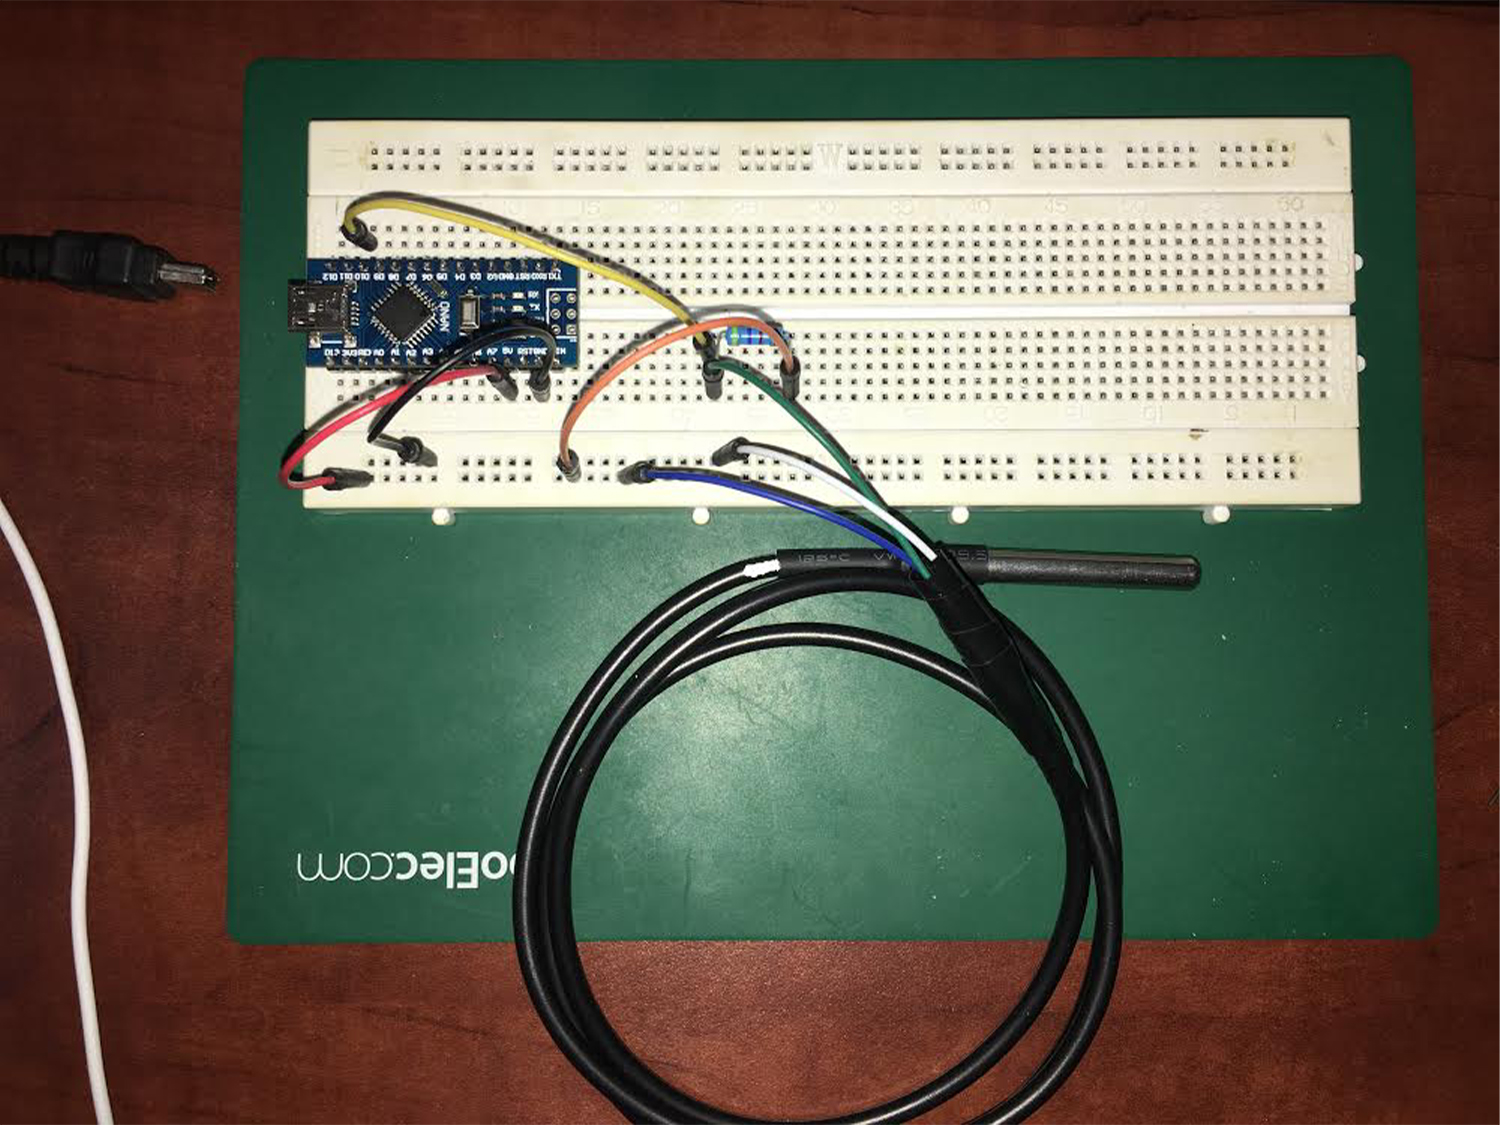
\includegraphics[width=0.65\linewidth]{pruebas1.jpg}
	\caption{Conexión Sencilla entre Arduino Nano y Sensor de Temperatura DS18B20}
\end{figure}

\par \noindent
En la imagen anterior hemos seleccionado el pin digital 10 para enviar la información y vemos como el sensor es conectado a la salida de 5V del Arduino y su respectivo GND, adicional vemos una resistencia de 4.7K entre el cable de DATA del sensor y una conexión al pin 10. 

\par \noindent
Ahora utilizando el software platformio, el entorno de desarrollo que utilizaremos para programar la placa Arduino, escribiremos un código de prueba. Para ellos necesitaremos de dos librerías: OneWire \cite{onewire-github} y DallasTemperature \cite{dallas-github}. El código de prueba sería el siguiente: \\

\begin{lstlisting}[language=C++, caption={Código Ejemplo para DS18B20}, captionpos=b]
#include <Arduino.h>
#include <OneWire.h>
#include <DallasTemperature.h>

#define ONE_WIRE_BUS 10

OneWire oneWire(ONE_WIRE_BUS);
DallasTemperature sensors(&oneWire);

void setup(){
Serial.begin(9600);
sensors.begin();
}


void loop(){
Serial.print("Requesting temperatures...");
sensors.requestTemperatures(); 
Serial.println("DONE");
Serial.print("Temperature:");
Serial.println(sensors.getTempCByIndex(0));
delay(1000);
}
\end{lstlisting}

\par \noindent
El código anterior puede ser encontrado como uno de los ejemplos que trae la librería DallasTemperature[30] bajo el nombre "Simple.pde" y puede inspeccionado por cualquier editor de texto. El código básicamente es crear una instancia de la clase OneWire y esa instancia colocarla como argumento dentro del objeto "sensors". En la función setup (se ejecuta una sola vez). Se inicializa el puerto serial a 9600 baudios y se inicializa el objeto "sensors" de clase DallasTemperatures. En la función loop, se ejecuta toda la función, desde el inicio hasta el  final, una y otra vez; hasta que se apague el microcontrolador. Se imprime en la terminal de la computadora y se ejecuta la función "requestTemperatures" que llama todos los posibles DS18B20 que se encuentren en el mismo bus. Por último, se imprime en la terminal de la computadora el resultado de la función "getTempCByIndex" donde si está conectado un DS18B20 retorna la temperatura captura en grados Celsius; en caso tal de no encontrarse ningún DS18B20 en el circuito, el valor retornado es "-127" constante de definida en la librería DallasTemperature.

\par \noindent
Una vez hayamos subido el codigo a nuestro Arduino, debemos validar que el sensor funcione correctamente, pero ¿cómo? Conectado el Arduino a nuestra computadora utilizaremos el puerto serial de nuestro entorno de desarrollo. Si estamos utilizando el IDE de Arduino, basta con hacer clic en la barra superior la opción "herramientas" y seleccionar "Monitor Serial". Como nosotros estamos utilizando Platformio como IDE, basta con seleccionar en la barra de herramientas "Platformio", la opción "Serial Monitor". Esencialmente lo que hace esa opción es escribir en nuestra terminal el comando "pio device monitor  port COM5" y con eso podemos comunicarnos con nuestro Arduino a través de un puerto Serial. En la  gura 4.2, podemos visualizar el resultado del código 4.1, en ejecución por el microcontrolador.

\begin{figure}[H]
	\centering
	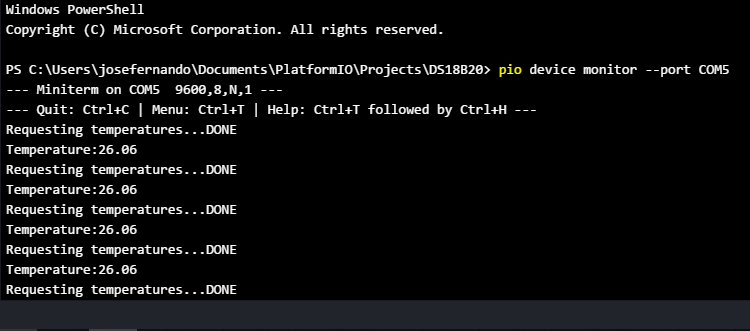
\includegraphics[width=\linewidth]{pruebas2.png}
	\caption{Terminal de Windows visualizando temperatura capturada por sensor DS18B20, a través de comunicación serial.}
\end{figure}

\par \noindent
Hemos comprobado lo sencillo que es capturar mediciones de temperatura en tiempo real. Sin embargo, no es práctico para el usuario final tener que cargar una computadora, conectar el Arduino y abrir una terminal. Aquí es donde necesitamos la pantalla LCD ILI9348.

\subsubsection{Arduino y Pantalla LCD ILI9341}
\par 
La realidad es que los datasheets de las pantallas LCD son complejas, esto es debido a que se explica más como el controlador de la pantalla interactúa con el LCD. Lo único que pudimos determinar es que la pantalla tolera una alimentación de 5V; pero, el controlador solamente utiliza una lógica de 3.3V. Teniendo en cuenta esto procedimos a conectar la pantalla utilizando divisores de voltaje (resistencias en serie); no obstante, el resultado no fue positivo.

\par \noindent
Por suerte el blog de educ8s.tv\cite{edu8tv} tiene una guía para utilizar la pantalla ILI9341,curiosamente utiliza resistores de 10K en series para las conexiones, a pesar de que las resistencias en serie no disminuyen el voltaje de los pines de Arduino. Conectamos la pantalla LCD ILI9341 a nuestro Arduino según la guía, quedando como se ve en la  gura 4.3

\par \noindent
El controlador de esta pantalla utiliza el bus SPI del Arduino, SPI por sus siglas en inglés es Serial Pheripheral Interface, el cual es un interfaz de bus comúnmente utilizado para enviar información entre microcontroladores, sensores, tarjetas SD y otros microcontroladores. Esto quiere decir que las conexiones de nuestra pantalla están definidas hacia los pines digitales 13, 12 y 11 para poder comunicarse correctamente con el Arduino.

\begin{figure}[H]
	\centering
	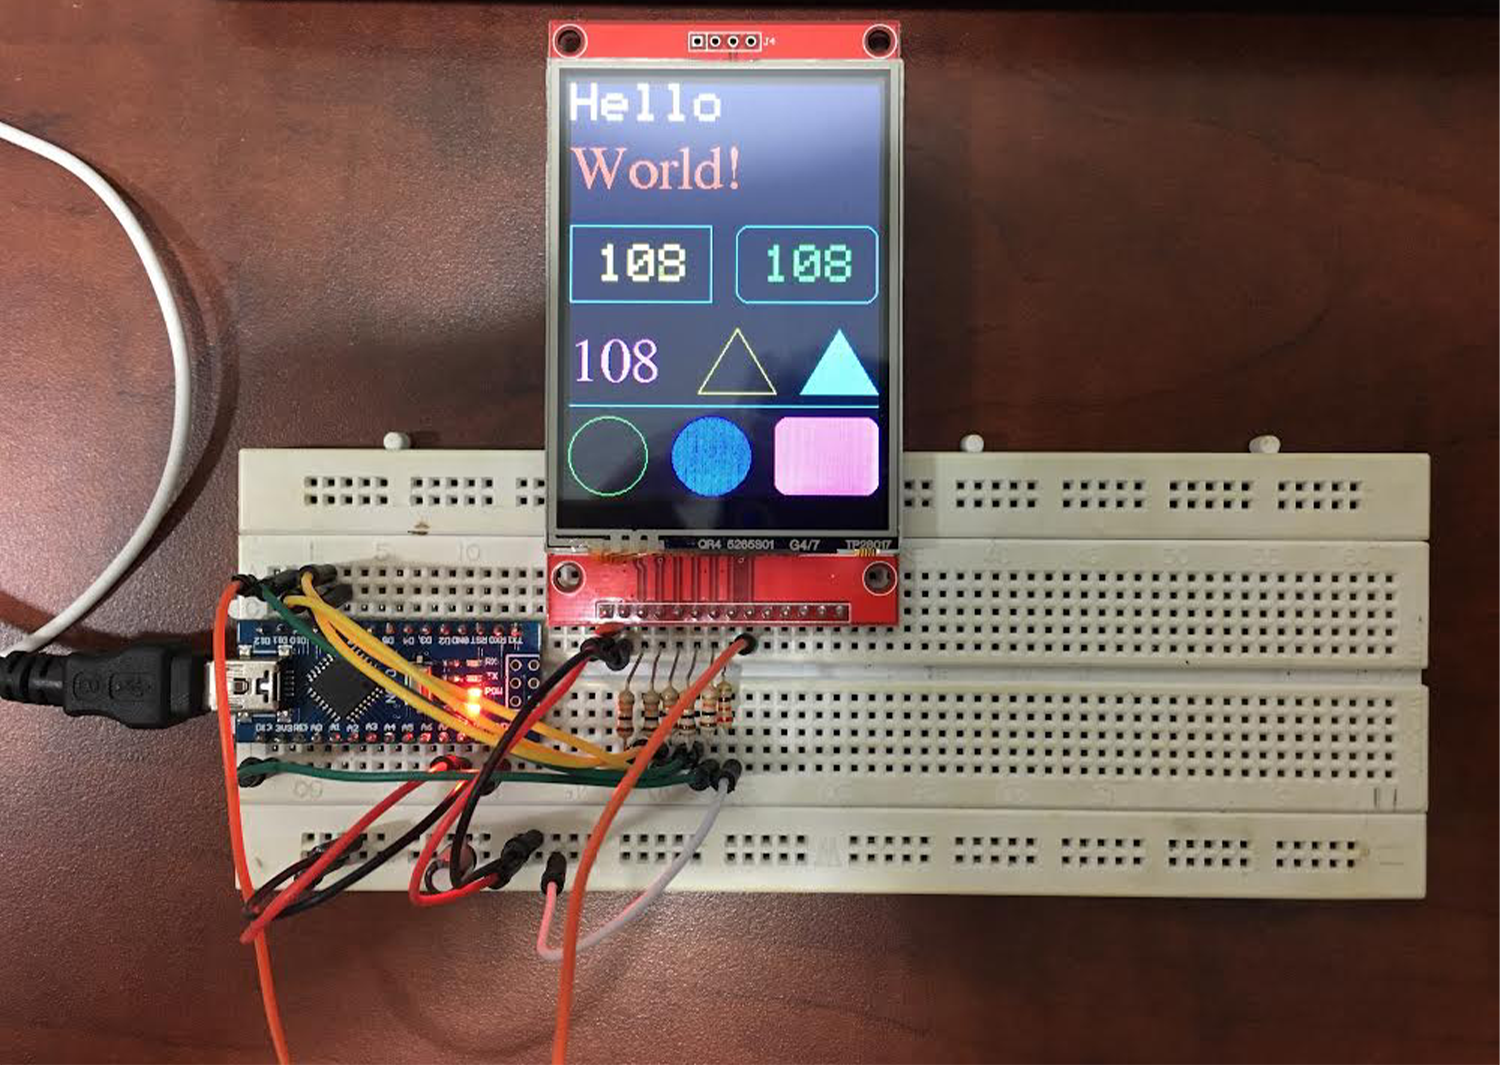
\includegraphics[width=0.8\linewidth]{pruebas3.png}
	\caption{Conexión entre Arduino y LCD ILI9341, utilizando resistencias de 10K en serie.}
\end{figure}

\clearpage

\par \noindent
Cabe a destacar que el circuito de la figura 4.3, utiliza dos componentes pasivos adicionales a las resistencias. Estos son dos capacitores, uno electrolítico de 10 uF, ayuda a filtrar frecuencias bajas y otro de cerámica de 1nF el cual ayuda a filtrar altas frecuencias. El conjunto de ambos brinda una fuente de poder estable a la pantalla LCD.

\par \noindent
La pantalla cuando es conectada al Arduino solamente despliega la luz de fondo blanca de la pantalla. Para programar los pixeles a utilizar en la pantalla debemos utilizar dos librerías: Adafruit\_ILI9341\cite{adafruit-lcd} y Adafruit-GFX-Library\cite{adafruit-gfx} ambos de los mismos desarrolladores de Adafruit, es una compañía de hardware de código abierto y es uno de los principales contribuidores del proyecto Arduino. Utilizamos uno de los códigos ejemplos que vienen con las librerías para verificar el funcionamiento de la pantalla como en la figura 4.3

\begin{lstlisting}[language=C++, caption={Codigo Ejemplo para pantalla LCD ILI9341}, captionpos=b]
#include <Arduino.h>
#include "SPI.h"
#include "Adafruit_GFX.h"
#include "Adafruit_ILI9341.h"

#define TFT_DC 9
#define TFT_CS 10
#define TFT_RST 8
#define TFT_MISO 12
#define TFT_MOSI 11
#define TFT_CLK 13

Adafruit_ILI9341 tft = Adafruit_ILI9341(
TFT_CS, 
TFT_DC, 
TFT_MOSI, 
TFT_CLK, 
TFT_RST, 
TFT_MISO);

#include <Fonts/FreeSerif24pt7b.h>

int Variable1;  

void setup(){

tft.begin();
tft.fillScreen(0x0000);
tft.setTextWrap(false);

tft.setCursor(0, 0);
tft.setTextColor(0xFFFF);
tft.setTextSize(4);
tft.println("Hello");

tft.setFont(&FreeSerif24pt7b);
tft.setTextSize(0);

tft.setCursor(0, 80);
tft.setTextColor(0xF800);
tft.println("World!");

tft.setFont();

tft.drawRect(0, 110, 110, 60, 0x07FF);
tft.drawRoundRect(129, 110, 110, 60, 10, 0x07FF);
tft.drawTriangle(100,240,    130,190,    160,240, 0xFFE0);
tft.fillTriangle(179,240,    209,190,    239,240, 0x07FF);
tft.drawLine(0, 250, 239, 250, 0x07FF);
tft.drawCircle(30, 289, 30, 0x07E0);
tft.fillCircle(110, 289, 30, 0x001F);
tft.fillRoundRect(160, 259, 80, 60, 10, 0xF81B);

}

void loop(){

Variable1++;
if(Variable1 > 150)
{
Variable1 = 0;
}

char string[10];

dtostrf(Variable1, 3, 0, string);

tft.setCursor(21, 125);
tft.setTextColor(0xFFE0, 0x0000);
tft.println(Variable1);

if(Variable1 < 10)
{
tft.fillRect(44, 124, 24, 34, 0x0000);
}
if(Variable1 < 100)
{

tft.fillRect(69, 124, 24, 34, 0x0000);
}

tft.setCursor(150, 125);
tft.setTextColor(0x07E0, 0x0000);
tft.setTextSize(4);
tft.println(string);

tft.fillRect(0, 198, 75, 34, 0x0000);

tft.setFont(&FreeSerif24pt7b);
tft.setTextSize(0);


tft.setCursor(0, 230);
tft.setTextColor(0xF81F);
tft.println(Variable1);


tft.setFont();
}
\end{lstlisting}

\par \noindent
Como podemos apreciar en el código 4.2 todas las funciones hacen referencia a la instancia de la clase "Adafruit\_ILI9341". Básicamente se puede pintar pixel por pixel la pantalla utilizando esta clase; sin embargo, ya hay funciones para realizar figuras geométricas como: "drawLine", "drawCircle", "drawTriangle" y "drawRect". Las funciones principales  son la de "fillscreen" la cual rellena la pantalla de un solo color y "println" el cual permite imprimir en la pantalla LCD como si fuese una terminal. En el ejemplo para seleccionar los colores del texto utilizaron números hexadecimales; pero, la librería cuenta con constantes para los colores más comunes.

\par \noindent
Solamente con el sensor de temperatura DS18B20 y la pantalla LCD ILI9341, es suficiente para realizar un prototipo. Ya que entra en la definición de lo que es un termómetro. El valor agregado a nuestro prototipo es la capacidad de poder comunicarse entre varios prototipos de manera simultánea, con el fin que uno de ellos sea el que envié la información de las mediciones de temperatura de todos los prototipos conectados a la aplicación en Android. Esta comunicación debe ser inalámbrica y el módulo de transmisión de radiofrecuencia es el encargado de dicha tarea.

\subsubsection{Arduino y Modulo nRF24L01+}
\par 
Durante el desarrollo de nuestro prototipo se llegó a la siguiente pregunta ¿Cómo envió de manera inalámbrica los datos capturados de temperatura de cada uno de los prototipos a mi smartphone? Llegamos a 3 opciones:

\begin{enumerate}
	\item Bluetooth
	\item Wi-fi
	\item RadioFrecuencia
\end{enumerate} 

\par \noindent
Rápidamente descartamos utilizar Bluetooth, este estándar de transmisión de información inalámbrica requiere en la mayoría de sus versiones una comunicación exclusivamente de dos dispositivos. Un dispositivo actuando como maestro y el otro como esclavo. La idea es conectar múltiples prototipos con nuestro smartphone. 

\par \noindent
Después pasamos a utilizar tecnología Wi-Fi, nuestros smartphones tienen antenas de Wi-Fi incorporadas y podemos agregar módulos como el ESP8266, que en realidad es un microcontrolador con capacidades inalámbricas. Sin embargo, estos módulos tienen un consumo moderado a alto de energía, el cual nuestro Arduino no puede satisfacer de manera consistente y disminuiría el tiempo de operación de nuestro prototipo.

\par \noindent
Nuestra última opción es Radio Frecuencia, ya que es muy parecido a utilizar un módulo Wi-Fi, es más prácticamente se encuentran en la misma banda de 2.4 GHz. La ventaja de utilizar esta tecnología es que su consumo de energía es mínimo, por lo que puede ser conectado a un Arduino sin problemas. Otra y quizás la más importante es que los módulos nRF24L01+ cuentan con una característica llamada "MultiCeiver", esta característica permite a un solo modulo actuando como receptor comunicarse con hasta 6 otros módulos actuando como transmisión de manera paralela.  La desventaja es que la mayoría de los smartphones no cuentan con un transceptor compatible con radio frecuencia. Teniendo en cuenta esta limitante se designó utilizar esta tecnología para la comunicación entre los prototipos solamente. 

\par \noindent
Los prototipos todos contarían con un chip de radio frecuencia nRF24L01+; pero solo un prototipo sería el encargado de enviar la información de todos los otros prototipos a él smartphone. 

\par \noindent
El módulo nRF24L01+ requiere de la alimentación del pin de salida 3.3V del Arduino. Adicional requiere dos pines digitales para que el Arduino asigne si el módulo funcionara como transmisión o recepción. Por último, este módulo utiliza el mismo bus que la pantalla LCD ILI9341, la interfaz de bus que se menciona es SPI y por defecto se encuentra en los pines 13, 11 y 12 de nuestro Arduino. 

\begin{figure}[H]
	\centering
	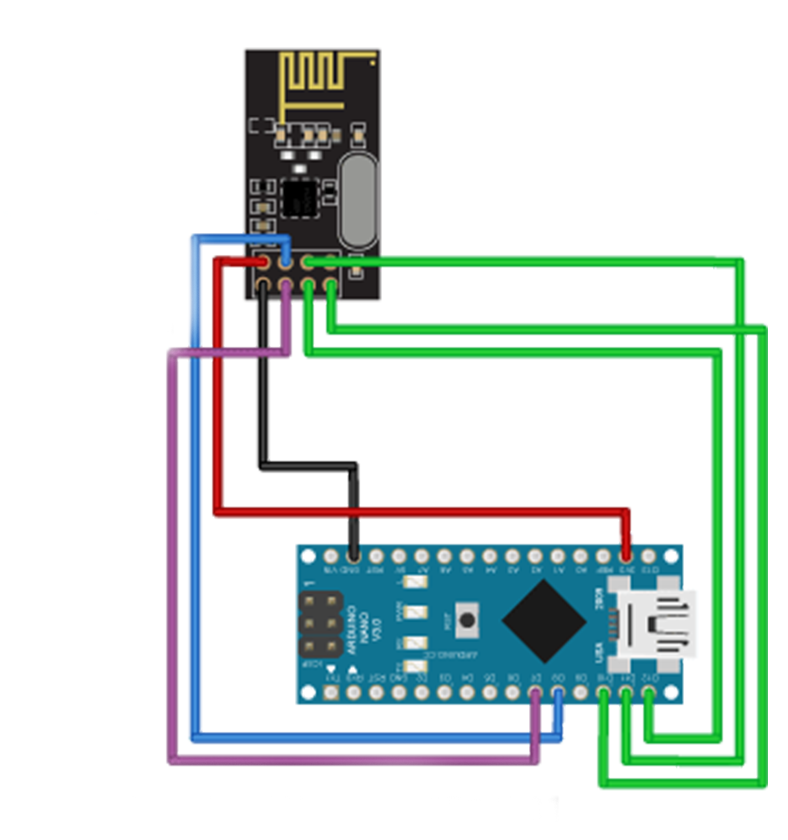
\includegraphics[width=0.5\linewidth]{pruebas4.png}
	\caption{Ejemplo de cómo conectar el módulo nRF24L01+ con un Arduino nano.}
\end{figure}

\par \noindent
Para programar este módulo con Arduino es necesario dos librerías: RF24\cite{rf24} y el SPI este último es una de las librerías por defecto que trae Arduino. Dentro de las librerías encontramos un código ejemplo llamado "GettingStarted.ino", es un ejemplo básico de como enviar información de un módulo a otro.

\clearpage

\begin{lstlisting}[language=C++, caption={Codigo Ejemplo para módulo nRF24L01+}, captionpos=b]
#include <Arduino.h>

#include <DigitalIO.h>
#include <SPI.h>
#include "RF24.h"

bool radioNumber = 1;

RF24 radio(4,5);

byte addresses[][6] = {"1Node","2Node"};

bool role = 0;

void setup() {
	Serial.begin(115200);
	Serial.println(F("RF24/examples/GettingStarted"));
	Serial.println(
	F("*** PRESS 'T' to begin transmitting to 
	the other node"));
	
	radio.begin();
	radio.setPALevel(RF24_PA_MAX);
	
	if(radioNumber){
		radio.openWritingPipe(addresses[1]);
		radio.openReadingPipe(1,addresses[0]);
	}else{
		radio.openWritingPipe(addresses[0]);
		radio.openReadingPipe(1,addresses[1]);
	}
	
	radio.startListening();
}

void loop() {

	if (role == 1)  {
	
		radio.stopListening();                                    
		
		
		Serial.println(F("Now sending"));
		
		unsigned long start_time = micros();                      
		if (!radio.write( &start_time, sizeof(unsigned long))){
		Serial.println(F("failed"));
		}
		
		radio.startListening();                                   
		
		unsigned long started_waiting_at = micros();              
		boolean timeout = false;                                  
		
		while ( ! radio.available() ){                            
			if (micros() - started_waiting_at > 200000 ){           
				timeout = true;
				break;
			}
		}
		
		if ( timeout ){                                           
			Serial.println(F("Failed, response timed out."));
		}else{
			unsigned long got_time;                               
			radio.read( &got_time, sizeof(unsigned long) );
			unsigned long end_time = micros();
			
			Serial.print(F("Sent "));
			Serial.print(start_time);
			Serial.print(F(", Got response "));
			Serial.print(got_time);
			Serial.print(F(", Round-trip delay "));
			Serial.print(end_time-start_time);
			Serial.println(F(" microseconds"));
		}
		
		delay(1000);
	}
	
	if ( role == 0 ){
		unsigned long got_time;
		
		if( radio.available()){
		
			while (radio.available()){                                  
				radio.read( &got_time, sizeof(unsigned long) );            
			}
			
			radio.stopListening();                                       
			radio.write( &got_time, sizeof(unsigned long) );             
			radio.startListening();                                      
			Serial.print(F("Sent response "));
			Serial.println(got_time);
		}
	}
		
		if ( Serial.available() ){
		char c = toupper(Serial.read());
		if ( c == 'T' && role == 0 ){
		Serial.println(
		F("*** CHANGING TO TRANSMIT ROLE -- 
		PRESS 'R' TO SWITCH BACK"));
		role = 1;                 
		
		}else
		if ( c == 'R' && role == 1 ){
		Serial.println(F("*** CHANGING TO RECEIVE ROLE -- 
		PRESS 'T' TO SWITCH BACK"));
		role = 0;                
		radio.startListening();
		}
	}

} 
	
\end{lstlisting}

\par \noindent
El código 4.3 permite controlar el módulo nRF24L01+ a través del puerto serial de nuestra computadora. En el código se define el radioNumber, un módulo debe ser 0 y el otro 1, una instancia de la clase RF24 cuyos argumentos son los dos pines digitales del Arduino. Un arreglo de tipo byte que básicamente es la dirección que se le asigna a cada módulo y una variable de rol. 

\par \noindent
Al iniciar el programa abrimos el puerto serial con 115200 baudios, esto permite a nuestro Arduino a enviar más caracteres por el puerto serial a que si usáramos 9600. 

Iniciamos la instancia radio y utilizamos la función "setPALevel" donde programamos el amplificador de poder del módulo, se utiliza como argumento "RF24\_PA\_MAX" el cual es el valor más alto que acepta nuestro módulo. Seguido de una sentencia if, donde dependiendo del Arduino que se esté usando se abre una "tubería de comunicación" con el otro Arduino a través del módulo, una "tubería" se usa para enviar información y otro para recibir.

\par \noindent
La función loop cuenta de dos partes. Una son las sentencias que indican el rol del Arduino, recordemos que al inicio ambos Arduinos inician con el rol 0. Si un Arduino tiene en la variable "role" el valor 0, se encuentra en el modo de receptor donde espera un mensaje del otro módulo para enviar una respuesta. En caso contrario y la variable "role" tiene el valor 1, entonces el módulo envía un mensaje al otro módulo y espera la respuesta del mensaje enviado. Esto permite una comunicación bilateral y da más control al Arduino de cómo manejar la información.

\par \noindent
La segunda parte básicamente el Arduino está a la espera de recibir a través del puerto serial, terminal de nuestra computadora, los valores 'T' o 'R'. En caso tal que el usuario escriba 't' o 'T', el Arduino le envía un mensaje al usuario que ha cambiado a modo de transmisión o sea el "role" ahora tiene un valor de 1. Si el usuario escribe 'r' o 'R' entonces nuevamente se envía un mensaje para notificar al usuario y se asigna el valor de "role" a 0. En caso de que el usuario ingrese cualquier otra cosa no pasa nada. Recordemos que la función "loop" se ejecutara una y otra vez, mientras que el Arduino tenga una fuente de poder.

\begin{figure}[H]
	\centering
	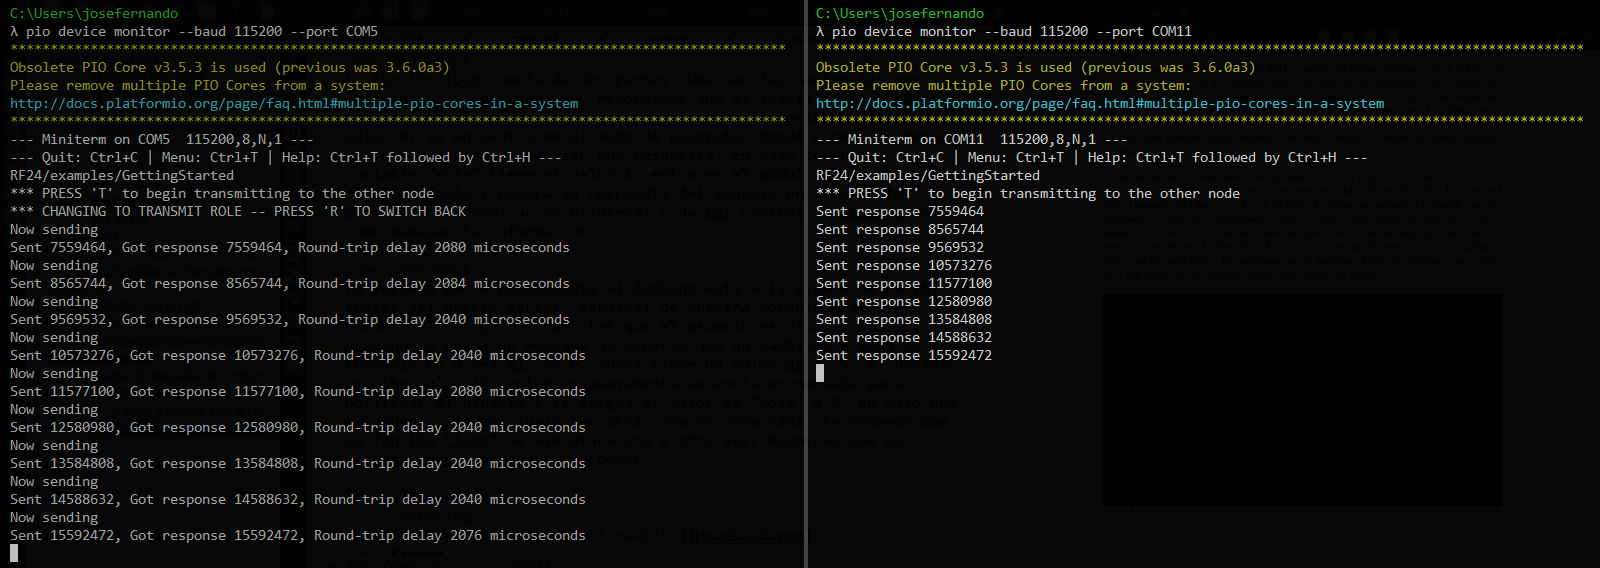
\includegraphics[width=\linewidth]{pruebas5.png}
	\caption{Resultado del código 4.3, dos Arduino comunicándose de manera bilateral utilizando los módulos nRF24L01+.}
\end{figure}

\par \noindent
El módulo nRF24L01+ brinda gran valor para nuestro prototipo por su poco precio; sin embargo, la característica que falta es enviar la información de todos los sensores a nuestro smartphone. Aquí es donde necesitamos el módulo bluetooth HC-05.  

\subsubsection{Módulo Bluetooth HC-05}



